\documentclass[11pt,xcolor=svgnames]{beamer}
\usepackage{dsfont,natbib,setspace,changepage,multirow}
\mode<presentation>

% replaces beamer foot with simple page number
\setbeamertemplate{navigation symbols}{}
%\setbeamerfont{frametitle}{series=\bfseries}
\setbeamercolor{frametitle}{fg=Black}

\setbeamertemplate{footline}{
   \raisebox{5pt}{\makebox[\paperwidth]{\hfill\makebox[20pt]{\color{gray}\scriptsize\insertframenumber}}}}

\usepackage{algorithm}
\usepackage{algorithmic}

% colors
\newcommand{\theme}{\color{Maroon}}
\newcommand{\bk}{\color{black}}
\newcommand{\rd}{\color{DarkRed}}
\newcommand{\fg}{\color{ForestGreen}}
\newcommand{\bl}{\color{blue}}
\newcommand{\gr}{\color{black!50}}
\newcommand{\sg}{\color{DarkSlateGray}}
\newcommand{\nv}{\color{Navy}}
\setbeamercolor{itemize item}{fg=gray}

% common math markups
\newcommand{\bs}[1]{\boldsymbol{#1}}
\newcommand{\mc}[1]{\mathcal{#1}}
\newcommand{\mr}[1]{\mathrm{#1}}
\newcommand{\bm}[1]{\mathbf{#1}}
\newcommand{\ds}[1]{\mathds{#1}}
\newcommand{\indep}{\perp\!\!\!\perp}
\def\plus{\texttt{+}}
\def\minus{\texttt{-}}

% spacing and style shorthand
\setstretch{1.1}

\begin{document}

\setcounter{page}{0}
{ \usebackgroundtemplate{
\includegraphics[height=\paperheight]{phoenix}}
\begin{frame}[plain]
\begin{center}

{\bf \LARGE \theme }

{\bf \Large  Making Decisions in High Dimensions}

\vskip 2cm
Matt Taddy,  Chicago Booth


\vskip .25cm
{\texttt{faculty.chicagobooth.edu/matt.taddy/research}}

\end{center}
\end{frame} }


\begin{frame}

{\bf High Dimensional Decisions}

\vskip .5cm
One of the ways that data is `Big' is in the {\theme number of inputs}.

\vskip .25cm
This number often {\theme grows with the sample size} (e.g., words in text, websites in browsers) and you never reach a statistically safe place.

\vskip .5cm
For this type of Big, we need {\nv dimension reduction} techniques: project from the full input set down to a useful low-D summary.

\vskip .25cm
Crucially, this must be focused on the {\nv decisions} you'd like to make.

\end{frame}


\begin{frame}

{\bf Fancy plot: \bk monthly stock returns}

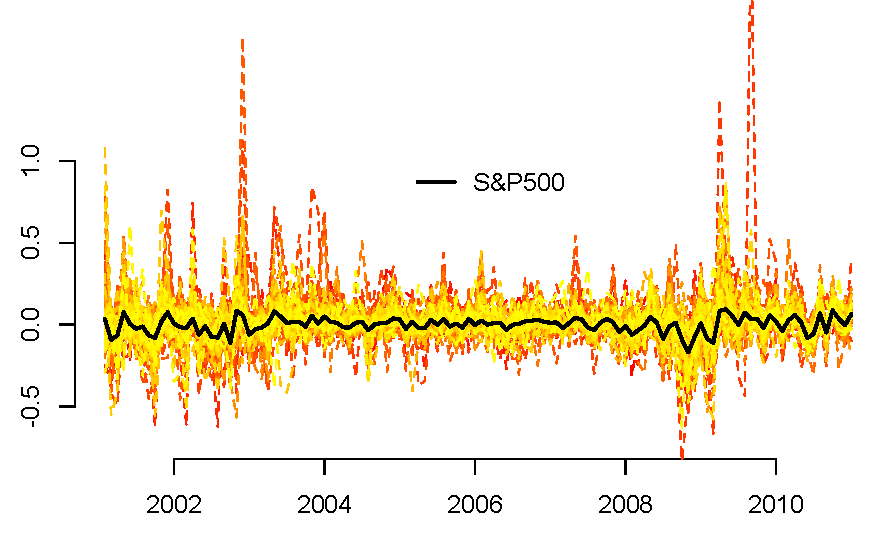
\includegraphics[width=4.25in]{graphs/fancyret}

\vskip .25cm
\hfill{\nv What do we learn?}

\vskip -.5cm
\end{frame}



\begin{frame}

{\bf Useful plot: \bk market model coefficients}

\vskip .25cm
Fit a line between stock returns $R_t$ and market returns $M_t$ (SP).
\[
R_t \approx \alpha + \beta M_t
\]
$\alpha$ is money you make regardless of what the market does.\\
$\beta$ is the asset's sensitivity to broad market movements.

\begin{center}
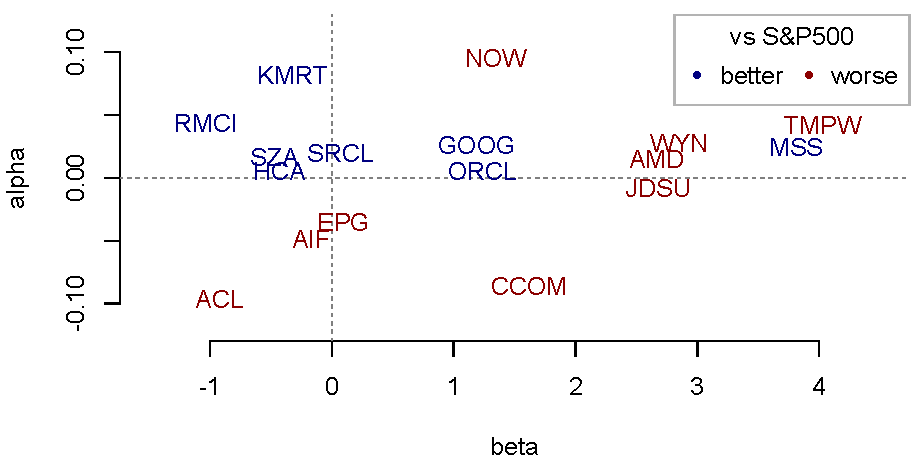
\includegraphics[width=3.5in]{graphs/usefulret}
\end{center}
\vskip -1cm
\end{frame}



\begin{frame}

Many problems in BD involve a response of interest
(`{\theme y}')\\ and a set of covariates (`{\theme \bf x}') to
be used for prediction.

\vskip .5cm
If your `decision' is to predict $y$ for new $\bm{x}$,  we need to {\nv reduce dimension} in the direction of $y$.  That is, we want to map $\bm{x}\rightarrow \hat y$.

\vskip .5cm
A general tactic is to deal in averages and lines.  \\
{We'll model the 
  conditional mean for y given {\bf x},}
\[\large
\ds{E}[~ y \mid \bm{x} ~] = f( \bm{x}'\bs{\beta} )
\]

$\bm{x} = [1, x_1, x_2,\ldots x_p]$  is your vector of
    covariates.\\
\vskip .2cm
$ \bs{\beta} = [\beta_0, \beta_1, \beta_2, \ldots \beta_p]$ are the corresponding
coefficients.

\end{frame}


\begin{frame}

{\bf Some basic facts about linear models}

\vskip .5cm
{The model is always $\ds{E}[y|\bm{x}] = f(\bm{x}\bs{\beta})$.}
\begin{itemize}
\item Gaussian (linear): $y \sim \mr{N}(\bm{x}\bs{\beta},\sigma^2)$. 
\item Binomial (logistic): $\mr{p}(y=1)= e^{\bm{x}\bs{\beta}}/(1+ e^{\bm{x}\bs{\beta}})$.
\end{itemize}

\vskip .4cm

Likelihood (LHD) is $\mr{p}(y_1|\bm{x}_1)\times\mr{p}(y_2|\bm{x}_2)\cdots\times\mr{p}(y_n|\bm{x}_n)$.

\vskip .2cm
The Deviance (dev) is proportional to -log(LHD).

\vskip .2cm
$\bs{\hat\beta}$ is commonly fit to maximize LHD $\Leftrightarrow$ minimize deviance.

\vskip .5cm
Fit is summarized by $R^2 = 
1 - \text{dev}(\bs{\hat\beta})/\text{dev}(\bs{\beta}=0)$.

\vskip .2cm

{\theme The only $R^2$ we ever really care about is out-of-sample $R^2$.}

\end{frame}


\begin{frame}

{\bf {\nv Example:} Semiconductor Manufacturing Processes}

\begin{columns}[c]

\column{1.75in}

\vskip .25cm

\includegraphics[width=2in]{graphs/schalfhigh}
\column{2in}\small
\begin{center}


Very complicated operation\\
{\sg Little margin for error.}


\vskip .25cm
Hundreds of diagnostics\\
{\sg Useful or debilitating?}

\vskip .25cm
We want to focus reporting and
better predict failures.

\end{center}

\end{columns}

\vskip .5cm
$\bm{x}$ is 200 input signals, $y$ has 100/1500 failures.

\vskip .25cm
Logistic regression for failure of chip $i$ is

\vspace{-.25cm}
\[p_i = \mr{p}({\tt fail}_i|\bm{x}_i) = e^{\alpha+\bm{x}_i\bs{\beta}}/(1+ e^{\alpha+\bm{x}_i\bs{\beta}})
\]


% The $x_{ij}$ inputs here are actually orthogonal: they are the first 200 Principal Component directions from an even bigger set.

\vspace{-.25cm}

\end{frame}

\begin{frame}


The full model has $R^2 = 0.56$ {\gr (based on {\it binomial} deviance)}.

The p-values for these 200 coefficients:


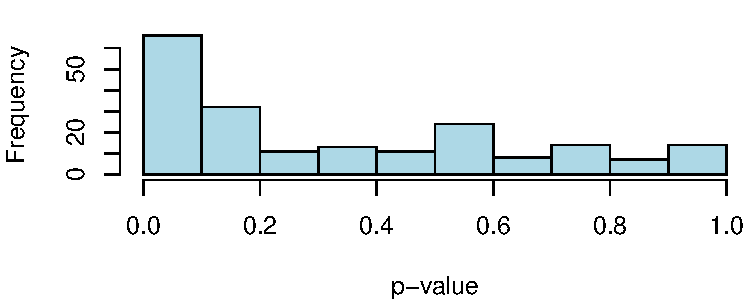
\includegraphics[width=4.1in]{graphs/SCpvals}

\vskip .25cm

{\gr Some are clustered at zero, the rest sprawl out to one.}\\

FDR of $q=0.1$ yields  $\alpha=0.0122$ p-value rejection cut-off. \\Implies 25 `significant', of which approx 22-23 are true signals.

\end{frame}


\begin{frame}


A {\it cut} model, using only these 25  signals,
has $R_{cut}^2 = 0.18$.  \\
This is much smaller than the full model's $R_{full}^2=0.56$.

\vskip .5cm
In-Sample (IS) $R^2$ {\it always} increases with more covariates.
\\ {\gr This is exactly what MLE $\bs{\hat\beta}$ is fit to maximize.}
\\ {\theme But how well does each model predict {\it new} data?}

\vskip .5cm
{ An out-of-sample (OOS) experiment}
\begin{itemize}
\item split the data into 10 random subsets {(`folds')}.
\item Do 10x: fit model $\bs{\hat\beta}$ using only 9/10 of data, 
\\ ~~~~~~~~~~~and record $R^2$ on the left-out subset. 
\end{itemize}
These OOS $R^2$ give us a sense of how well each \\model can predict
data that it has not already seen.
\end{frame}

\begin{frame}

We gain predictive accuracy by {\it dropping} variables.

\begin{center}\vspace{-.2cm}
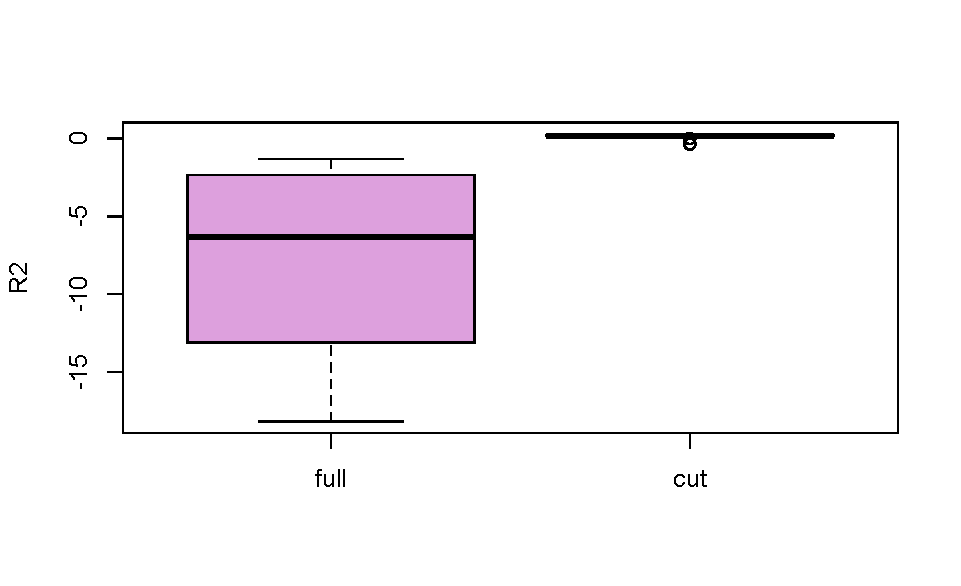
\includegraphics[width=4in]{graphs/SCr2}
\end{center}

Cut model has mean OOS R2 of 0.09, about 1/2 in-sample R2.

\vskip .2cm
The full model is terrible.  It is overfit and worse than $\bar y$.\\ 
{\nv Negative R2 are more common than you might expect.}

\vspace{-.2cm}
\end{frame}

\begin{frame}


{\nv All that matters is Out-of-Sample $R^2$.}  \\{\theme We don't care about In Sample $R^2$.}

\vskip .5cm
Using OOS experiments to  choose the best model is called {\it cross validation}.  It will be a big part of our big data lives.

\vskip .5cm
Selection of `the best' model is at the core of all big data.

\vskip .1cm
But before getting to selection, we first need strategies to \\ build good sets of candidate models to choose amongst.

\end{frame}



\begin{frame}

{\bf Regularization}

\vskip .5cm
The key to contemporary statistics is
{\nv regularization:} \\~~~~~~~~~~~~~~~depart from optimality to stabilize a system.

{\gr Common in engineering: I wouldn't drive on an optimal bridge.}

\vskip .5cm
We minimize deviance \onslide<2->{{\nv plus a cost on the size of
coefficients.}} {\large\begin{equation*}
\mr{min} 
-\frac{2}{n}\log \text{LHD}(\bs{\beta}) 
\onslide<2->{{\nv + \lambda\sum_k |\beta_k|}}
\end{equation*}}

\vskip -.25cm
\onslide<2>{This particular cost gives the `lasso': the new least squares.}

\end{frame}


\begin{frame}

{\bf Decision theory: \theme Cost in Estimation}

\vskip .5cm
Decision theory is based on the idea that choices have costs.\\
Estimation and hypothesis testing: what are the costs?


\vskip .5cm 
{\nv Estimation:}

\vskip .1cm
Deviance is the cost of distance between data and the model.\\
{\gr Recall: $\sum_i (y_i-\hat{y}_i)^2$ or 
$-\sum_i y_i\log(\hat{p}_i) - (1-y_i )\log(1-\hat{p}_i)$.}

\vskip .25cm
{\nv Testing:}

\vskip .1cm
Since $\hat{\beta}_j = 0$ is  {\it safe},  it should cost us to
decide otherwise.

\vskip .5cm 
$\Rightarrow$ The cost of $\hat{\beta}$ is deviance plus
a penalty  away from zero.



\end{frame}


\begin{frame}

{\bf{\gr [Sparse]}  Regularized Regression}


{\nv\large\[
\mr{min} \left\{ -\frac{2}{n}\log\text{LHD}(\bs{\beta}) + \lambda \sum_j c(\beta_j)\right\}
\]}

$\lambda >0$ is the penalty weight, $c$ is a cost (penalty) function.

$c(\beta)$ will be lowest at $\beta=0$ and we pay more for $|\beta| > 0$.

\vskip .1cm
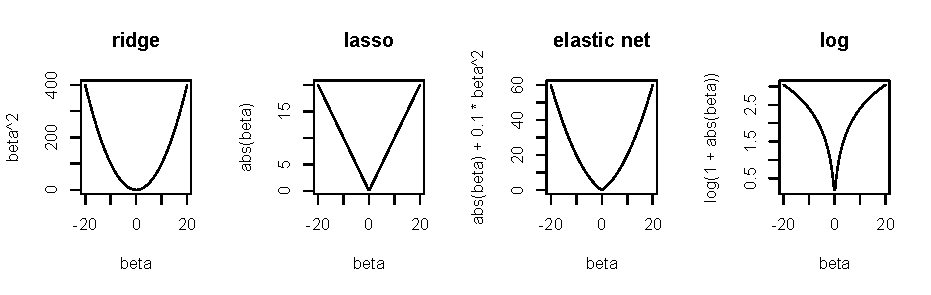
\includegraphics[width=4.25in]{graphs/penalties}

Options: ridge $\beta^2$, lasso $|\beta|$, elastic net $\alpha\beta^2 + |\beta|$,  $\log(1 + |\beta|)$.


\end{frame}


\begin{frame}

{\bf Penalization can yield {\theme automatic variable selection}}

The minimum of a smooth + pointy function can be at the point.

\vskip -.25cm
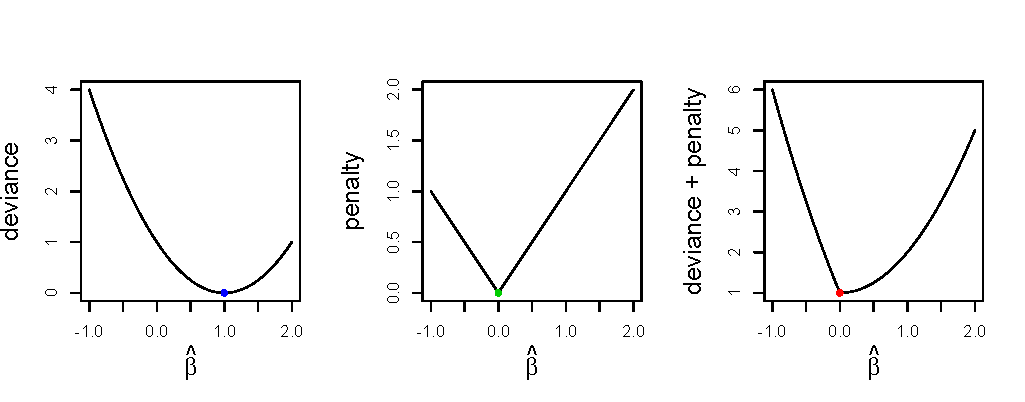
\includegraphics[width=4.25in]{graphs/penlasso}

\vskip .5cm
Anything with an absolute value (e.g., lasso) will do this.  

\vskip .1cm 
{\gr There are MANY penalty options and far too much theory.}

\vskip .1cm 
Think of lasso as a baseline, and others as variations on it.

\end{frame}

\begin{frame}

{\bf Lasso Regularization Paths}
\vskip .5cm

The lasso fits $\bs{\hat\beta}$ to minimize $-\frac{2}{n}\log\text{LHD}(\bs{\beta}) + \lambda \sum_j |\beta_j|$.

\vskip .1cm
We'll do this for a {\it sequence} of penalties $\lambda_1 > \lambda_2 ... > \lambda_T$.

\vskip .1cm
{\gr Then we can apply model selection tools to choose best $\hat \lambda$.}

\vskip .5cm
{\nv Path estimation:}

\vskip .1cm
~~~ Start with big $\lambda_1$ so big that $\bs{\hat \beta}=\bm{0}$.

\vskip .1cm
~~~ For $t=2\ldots T$: update $\bs{\hat \beta}$ to be optimal under $\lambda_t < \lambda_{t-1}$.

\vskip .5cm


Since estimated $\bs{\hat\beta}$ changes smoothly along this path:
\begin{itemize}
\item It's fast!  Each update is easy.
\item It's stable: optimal $\lambda_t$ may change a bit from sample to sample, but that won't affect the model much.
\end{itemize}

\end{frame}


\begin{frame}

The whole enterprise is easiest to understand visually.

\vskip -.25cm
\begin{center}
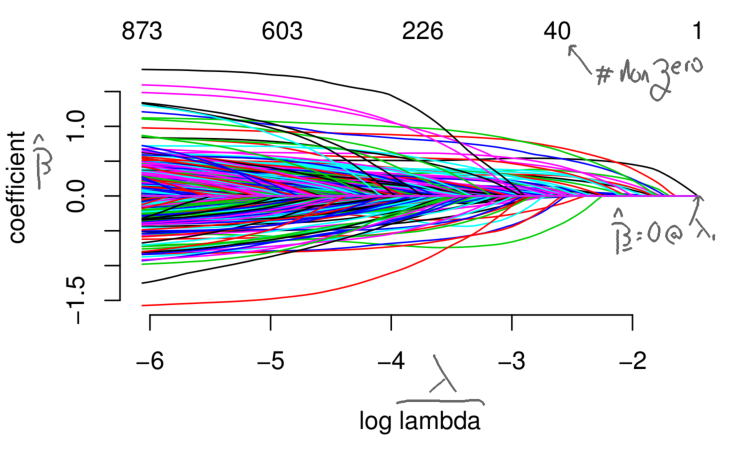
\includegraphics[width=.95\textwidth]{graphs/comscore_markeduppaths}
\end{center}

\vskip -.25cm
The algorithm moves {\it right to left}.  \\The $y$-axis is $\bs{\hat\beta}$ (each line a different $\hat\beta_j$) as a function of $\lambda_t$.
\end{frame}



\begin{frame}\

{\bf {\nv Example: } Comscore web browser data}

\vskip .5cm
The previous plot is  household log-online-spend regressed onto $\%$ of time spent on various websites (each $\beta_j$  a different site).

\vskip .25cm
Comscore records info on browsing\\ and purchasing behavior for annual panels of households.

\vskip .25cm
I've extracted 2006 data for the 1000 most heavily trafficked websites and for 10,000 households that spent at least 1\$.  


\vskip .25cm
Why do we care?  {\theme Predict consumption from browser history.}

\vskip .1cm
{
e.g., to control for base-level spending, say, in estimating advertising effectiveness.  
You'll see browser history of users when they land, but likely not what they have bought.  }

\vskip .5cm
{\sf\nv http://faculty.chicagobooth.edu/matt.taddy/teaching/comscore.R}
\end{frame}


\end{document}






























